\CHAPTER{Output Mode Cleaner}
\label{chapter4}
%\doublespace
\SECTION{Introduction}
Any fields present on the detection photodiode other than the signal
field and the local oscillator will lead to additional shot noise but
no additional signal: a degredation of SNR.  The additional fields can
be either distinct in frequency (such as the RF sidebands when using
DC readout) or in spatial mode. 

To remove these spurious fields, we employ an optical filter cavity at
the interferometer's output. This is the \emph{output mode cleaner}
(OMC).

\SECTION{General theory of mode cleaners}

Critically-coupled resonant cavities act as optical filters, allowing
the resonant mode to be transmitted while all orthogonal modes are
highly attenuated.  These cavities can be not only
frequency-selective, but also select a single spatial mode.

\begin{figure}[t]
\centerline{\includegraphics[width=\columnwidth]{figures/as_spot.png}}
\caption{\label{fig:as-spot}Image of the beam spot at the output port taken using a CCD
  camera. Although this image is saturated in the central portion, it
  shows the messy junk light surrounding the central gaussian beam.
  This includes contributions from both the carrier and the 25 MHz
  sidebands.}
\end{figure}

\SECTION{Eigenmodes}

A phase-front that returns to its original state after making a
round-trip through the optical cavity will interfere constructively
with itself, resonating in the cavity.  The set of such amplitude
distributions which are stable in the cavity and do not mix with one
another are collectively the \emph{eigenmodes} of the cavity.  The
eigenmodes of a cavity made with spherical mirrors are parametrized by
either the Hermite-Gauss or Laguerre Gauss modes.  These are the
energy eigenfunctions of the quantum harmonic oscillator.

The Hermite-Gauss modes are given by:

\begin{equation}
E_{nm}(x,y) = E_0 
\sqrt{ 
  \frac{2}{\pi w n! m! 2^n 2^m}
}
\exp \left\{-\frac{x^2+y^2}{w^2}\right\}
H_m\left( \frac{\sqrt{2}x}{w} \right)
H_n\left( \frac{\sqrt{2}y}{w} \right)
\end{equation}

\begin{figure}
\includegraphics[width=\columnwidth]{figures/hgmodes.pdf}
\caption{Hermite-Gauss modes. Positive amplitude is indicated in red and negative amplitude in blue.}
\end{figure}

\SECTION{Physical design of the cavity}

The output mode cleaner (OMC) consists of a four-mirror bowtie cavity
with a finesse of approximately 350. The cavity optics and detection
photodiodes are attached to tombstones which are bonded to a glass
slab. This entire optical bench is suspended by a double pendulum,
which in turn rests on an active seismic isolation platform, all of
which is contained within the vacuum envelope. For convenience the
chamber containing the OMC is isolated from the rest of the LIGO vacuum
envelope via a septum window, allowing the independent venting of
this chamber for easier access.

The output of the OMC is split via a 50/50 beamsplitter and directed
onto two high-quantum-efficiency InGaAs photodiodes. The two photodiode
signals allow the formation of sum and difference signals, the difference
providing a diagnostic `nullstream'.

%% Cavity properties [Table]
% These values are all from Sam's document T080144:
% https://dcc.ligo.org/cgi-bin/private/DocDB/ShowDocument?docid=5416
\begin{table}
\centering
\begin{tabular}{l l l l l}
\hline 
parameter          & design      & H1          & L1            & units   \\                    
\hline
perimeter ($p$)    & 1.042       & 1.077       & 1.016         & m       \\
beam waist ($w$)   & 477         & 496         & 463           & \micron \\
Finesse (\Finesse) & 400         & 360         & 360           &         \\
FSR                & 287.7       & 278.3       & 295.2         & MHz     \\  % fsr = c/p
cavity pole        & 360         & 390         & 410           & kHz     \\  % f_c = fsr/(2F)
g-factor           & 0.739       & 0.725       & 0.722         &         \\
HOM freq shift     & 69.4        & 67.2        & 71.8          & MHz     \\
transmission       & 1           & $\geq$0.95  & $\geq$0.90    &         \\
\hline
\end{tabular}
\caption{Designed and measured properties of the Hanford and Livingston output mode cleaners.}
\label{tab:OMCproperties}
\end{table}

\SECTION{Requirements}

The OMC is required to sufficiently filter the light present at the
output port such that contributions from the RF sidebands and higher-order
spatial modes become negligible. To exclude the RF sidebands, the
cavity length is chosen such that the RF sideband frequencies are
anti-resonant in the cavity, which yields minimum transmission.

\SECTION{Choosing the OMC finesse}

All things being equal, we want the best possible filtering capability
from the OMC.  

The transmission of a lossless critically-coupled cavity is given by
\begin{equation}
T = \frac{1}{1 + \frac{4}{\pi^2}\mathcal{F}^2\sin^2\phi}
\end{equation}
where $\mathcal{F}$ is the cavity finesse and $\phi$ is the cavity's
detuning from resonance.  Since the cavity will be locked to resonance
for the laser carrier, to find the attenuation of other modes, we set
$\phi$ to the detuning of these modes.

The maximum attenuation of a mode is given by $(4/\pi^2)\mathcal{F^2}$.

After filtering by the OMC, we want the shot noise contributions from
unneeded modes to be negligible, and the contribution from noises on
these fields to also be negligible.  Almost any cavity would be
sufficient to reduce excess shot noise contributions.  The need for a
high finesse OMC comes from the need to eliminate audio frequency
noises carried on the RF sidebands and higher-order spatial modes.

\begin{comment}
 h = 6.626068e-34;
 c = 299792458;
 lambda = 1064e-9;
 nu = c / lambda;
 P = 100e-3;
 shotnoise_RIN = sqrt(2*h*nu/P)
\end{comment}

Consider the contribution of intensity noise on the RF sidebands.  Any
residual intensity noise on the RF sidebands will contribute directly
to the DC readout signal.  Assume that the carrier has about 100 mW
power and that the RF sidebands have about the same amount of power,
and assume that the laser intensity noise is $10^{-7}$ RIN.  The shot
noise RIN on 100 mW is (per equation~\ref{eq:shotnoise-asd})
$\sqrt{2h\nu/P} \approx 2\times10^{-9}$.  Thus we need to attenuate
the RF sidebands by at least a factor of 100.

The RF sidebands will not be exactly anti-resonant in the cavity but
will actually lie at about $0.1 fsr$ away from the carrier.  Thus the
attenuation is diminished by approximately $\sin^{-2} (0.1 \pi)
\approx 10$.  So we need attenuation of 1000.  But we really want at
least a factor of 10 margin, so we'll want maximum attenuation of
10000. This means we need a finesse of at least 160.



\SECTION{Length control (LSC)}

The cavity length is locked through dither locking.  The fast PZT
actuator is dithered at 10 kHz and this signal is synchronously
demodulated in the transmitted light.  The bandwidth of the servo is
about 100 Hz.

\SECTION{Input beam control (ASC)}

Aligning the input beam to the OMC is a significant problem.  The OMC
can only clean the mode insofar as we can tell what mode we want to
keep.

Several OMC alignment schemes were implemented and utilized.

The simplest alignment control simply uses the two QPDs mounted on the
OMC breadboard.  This has the advantage of being very robust and not
requiring that the OMC already be locked, and so it is ideal for
initial alignment of the OMC before locking the cavity.  The QPD
alignment, however, has no notion of the ideal DC pointing of the beam
and is sensitive not just to the carrier, but also the RF sidebands.

A second alignment scheme is to dither the two steering mirrors each
in pitch and yaw, demodulate the OMC transmitted signal at these
frequencies, and feed back to the mirrors.  This produces an alignment
system which maximizes power transmitted through the OMC.  Because
this is a quadratic point, linear beam jitter coupling is nulled.

Junk light, however, will lead the dither alignment astray.

RF Wavefront sensing.  We did not really consider this.

AF IM WFS.  The same OMC length dither which is used to lock the cavity
length produces an audio-frequency sidebands of the OMC mode in
reflection.  The beats between this light and the light rejected from
the OMC on a pair of photodiodes can be used to produce alignment
error signals.

Beacon dither.  

SNR dither.  Nicolas's scheme.

\SECTION{Automatic gain control}

The optical gain of the interferometer naturally varies slowly as
alignment drifts and the thermal state of the mirrors changes.  The
over-all loop gain must be kept within a few dB of its nominal value
in order for the loop to remain stable.

Before S6 this was done by periodically running a script which
measured the loop gain and adjusted a digital gain to bring it to
nominal.

The flexibility of the realtime code generator allowed us to implement
an automatic gain control servo directly in the OMC front-end.  This
was a nice convenience. 

\SECTION{Residual fluctuations}

\SECTION{Optical characterization}

\SUBSECTION{Mode scan}

With the interferometer controlled using the heterodyne readout, the
Output Mode Cleaner can be used as a mode analyzer cavity by varying
the cavity length by at least a free-spectral-range. Because this
range is more than the fast PZT actuator, this is accomplished by
putting a large step into the thermal actuator. These mode scans can
address questions such as:
\begin{itemize}
\item How well aligned is the OMC?
\item How well mode-matched is the OMC?
\item How much carrier power is at the output port compared to sideband
power?
\item How well balanced are the RF sidebands?
\item How much junk light is present at the output port?
\item Are there any nasty modes near the 00 mode that will sneak through?
\item The horizontal/vertical mode separation
\end{itemize}
The mode scan cannot, by itself, distinguish carrier mode light from
the arms vs carrier mode junk light.


\SUBSECTION{Scattering}

From the output port, the interferometer appears almost perfectly
reflective.  Any light scattered by the output optics at a small angle
could scatter into the interferometer mode, reflect off of the
interferometer, and interfere with the other fields there.


\SECTION{Interferometer lock acquisition}

Initial lock acquisition of the Enhanced LIGO interferometers is the
same as in Initial LIGO. Once the interferometer is locked using the
heterodyne readout schemes, a DARM offset is introduced to allow carrier
light to be transmitted to the output port. The Output Mode Cleaner
is then locked to this carrier light. Once the OMC is locked to the
carrier, control of DARM is transferred to the DC readout system.
After this transition, a few other changes are made to engage the
OMC alignment servoes and to put the readout electronics into low
noise mode. At this point the interferometer has reached its operation
configuration and astrophysical data-taking ({}``science mode'')
begins.


\begin{figure}
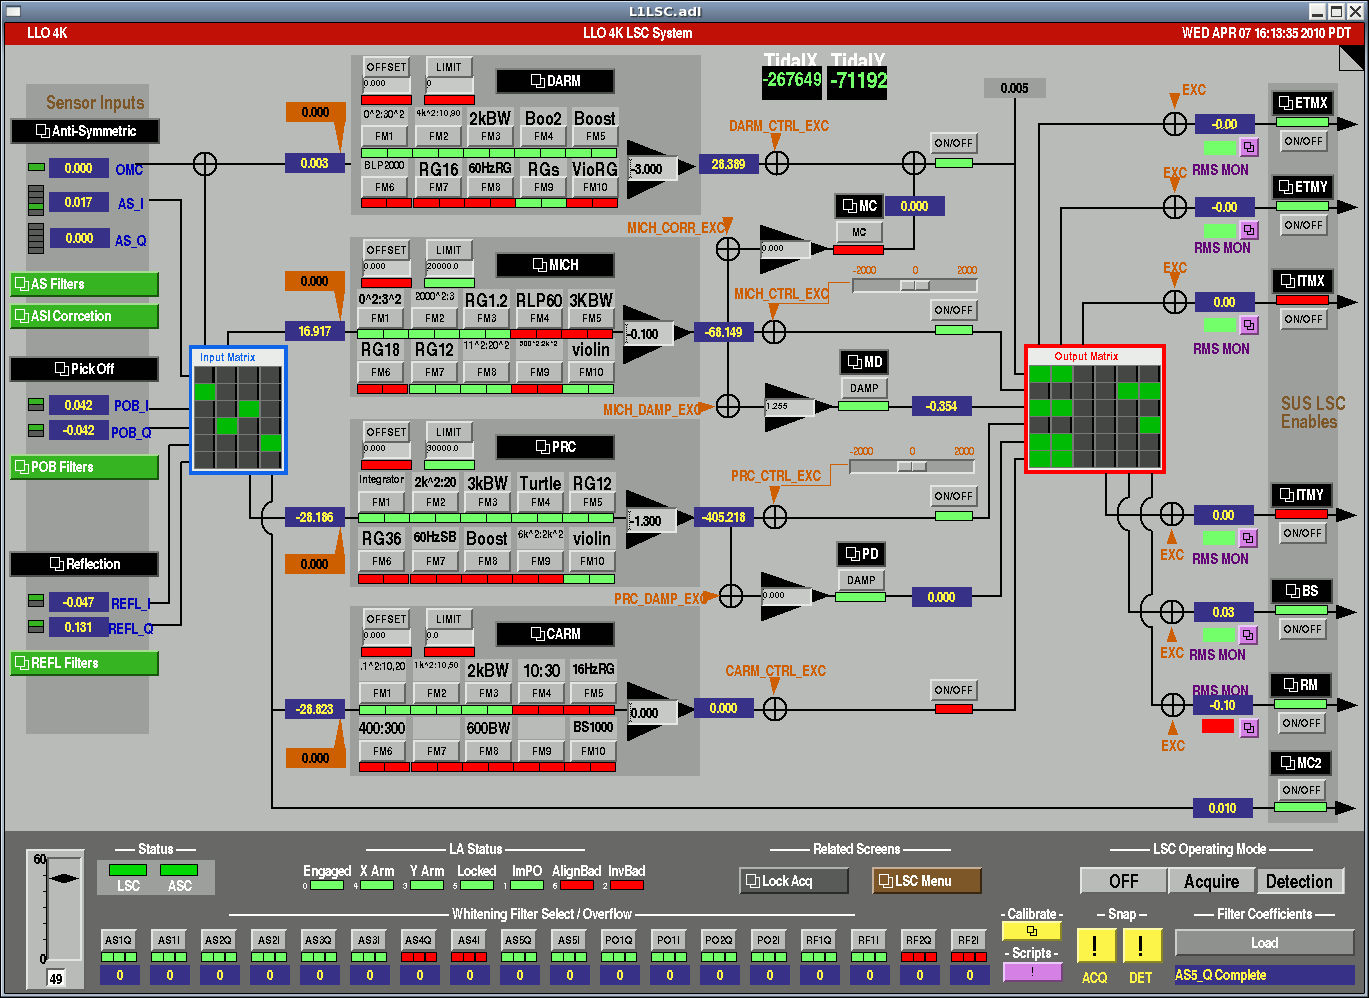
\includegraphics[width=\columnwidth]{figures/L1LSC.png}
\caption{The control screen for the Length Sensing and Control
  subsystem at Livingston.  The control screen depicts signal flow in
  a generally left-to-right manner.  Photodiodes at the anti-symmetric
  (AS), pick-off (PO), and reflected (REFL) ports are indicated on the
  extreme left.  These signals are combined via an input matrix to
  form the DARM, MICH, PRC, and CARM degrees of freedom.  These
  signals are processed through an array of filter banks defining the
  control filters.  Finally, the signals pass through an output matrix
  and are then directed to the individual optics.}
\end{figure}

\SECTION{Beam diverter}

When the interferometer loses lock, the stored power must be dumped
somewhere. Typically, due to the presence of the power recycling mirror,
the stored power comes out the output port. This high-power transient
is sufficiently strong to burn the detection photodiodes. In order
to prevent this, one of the steering mirrors is used as a fast shutter.
It is able to zero the transmission through the OMC in approx 2 ms.

\SECTION{The Front End}

\begin{quote}
\emph{Be exhorted:} you really can predict the noise floor accurately--to
accept a noisy front end is one of the stupidest and most expensive
mistakes you can make in designing sensitive optical
instruments. Measure it, and make sure you can explain every half
decibel. -- Phil Hobbs, \emph{Building Electro-Optical Systems} \cite{Hobbs2009Building}
\end{quote}
